\appendix

\section{Appendices}

\subsection{Manual validation} 
\label{manual}
We hired annotators fluent in the languages of the data to manually validate it. They had to mark instances where an error had occurred in the appositive detection, the detected appositive was not factual, or the entity had been incorrectly linked to WikiData (all instances of \textit{noise} in the data, resulting from errors in appositive detection and entity linking). Our ultimate goal was to build test sets of 1,000 instances per language per entity type, equally balanced between positive and negative instances, i.e. we needed 500 valid data instances per language per entity type. Based on a pilot study, we determined that noise levels for candidate appositives for \textsc{person} entities were approximately 33\% and for \textsc{organization} entities, 50\% (averaged across languages). We therefore gave annotators 750 and 1,000 candidates to annotate for the \textsc{person} and \textsc{organization} types, respectively. For most language-entity type combinations, the manual annotation successfully yielded close to 500 valid instances. That was not the case for Polish \textsc{organization} appositives, where only 80 valid candidates were retrieved, so we excluded this language-entity type combination from our work. It remains an open question whether \textsc{organization} appositives in Polish are rare or our automatic detection method failed at catching them. 

\subsection{Composition of cross-lingual data}
\label{composition}
Table~\ref{tab:facttypes} present findings on the composition of the Spanish, German and Polish positions of the data, respectively, as observed through cross-referencing with WikiData. The low number of facts for Polish is the result of one fact type dominating a large amount of the data (\textit{position held}).

\begin{table}[]
    \begin{subtable}{0.45\textwidth}
    \centering
    \small
    \begin{tabular}{clll}
                         &Fact type&News (\%)&Wiki(\%)\\
                         \hline                         %\multirow{10}{*}{\rotatebox{90}{\textsc{org-entity}}}&sovereign state&sovereign state\\
                         %&country&country\\
                         %&business&business\\
                         %&organization&big city\\
                         %&big city&\textcolor{gray}{enterprise}\\
                         %&political party&city\\
                         %&city&city 1000000+\\
                         %&city of the USA&political party\\
                         %&city 1000000+&\textcolor{gray}{capital}\\
                         %&university&\textcolor{gray}{landlocked country}\\
                         %\hline                         
                         \multirow{7}{*}{\rotatebox{90}{\textsc{per}}}&  position held & 20.9 & 9.4 \\ 
                          & occupation&15.9&10.6\\
                          & citizenship&10.1&4.3\\
                          & member of party&7.6&1.9\\
                          & award received&5.2&3.9\\
                          & nominated for&3.6&0.4\\
                          & educated at&3.1&3.1\\
                         \hline
                         \multirow{7}{*}{\rotatebox{90}{\textsc{org}}} & instance of&23.1&10.9\\
                         & official website & 6.3&6.2\\
                         & country&5.9&3.3\\
                         & member of&4.2&2.4\\
                         & subsidiary&3.5&2.1\\
                         & capital of&3.2&0.1\\
                         & has quality&3.0&0.0\\
    \end{tabular}
    \caption{English }
    \label{tab:wikidata}
    \end{subtable}
    \begin{subtable}{0.45\textwidth}
    \small
    \centering
    \begin{tabular}{clll}
                         &Fact type&News (\%)&Wiki(\%)\\
                         \hline                       \multirow{7}{*}{\rotatebox{90}{\textsc{per}}}&  position held&27.1&4.9\\
                          & occupation&11.2&10.3\\ 
                          & citizenship&9.8&4.8\\
                          & participant of&8.7&1.1\\
                          & member of party&7.3&1.3\\
                          & award received&4.1&3.2\\
                          & employer&3.2&0.5\\
                         \hline \multirow{6}{*}{\rotatebox{90}{\textsc{org}}} & instance of&28.9&10.5\\
                         & country&7.8&3.5\\
                         & has quality&5.1&0.1\\
                         & capital of&4.4&0.5\\
                         & member of&4.3&2.9\\
                         & is located in&3.4&2.2\\
    \end{tabular}
    \caption{Spanish }
    \label{Spanish}
    \end{subtable}
    \begin{subtable}{0.45\textwidth}
    \small
    \centering
    \begin{tabular}{clll}
                         &Fact type&News (\%)&Wiki(\%)\\
                         \hline                       \multirow{8}{*}{\rotatebox{90}{\textsc{per}}}&  position held&35.2&6.7\\
                          & employer&5.9&2.9\\ 
                          & citizenship&5.9&1.3\\
                          & member of party&5.3&2.4\\
                          & award received&4.9&2.1\\
                          & occupation&4.8&3.6\\
                          & participant of&4.6&1.5\\
                          & member of & 3.6&1.0\\
                         \hline \multirow{6}{*}{\rotatebox{90}{\textsc{org}}} & official website&15.6&12.4\\
                         & instance of&15.1&4.5\\
                         & owner of&7.5&2.4\\
                         & member of&5.8&0.9\\
                         & has quality&4.6&0.0\\
                         & Commons category&3.2&4.5\\
    \end{tabular}
    \caption{German }
    \label{German}
    \end{subtable}
    \begin{subtable}{0.45\textwidth}
    \small
    \centering
    \begin{tabular}{clll}
                         &Fact type&News (\%)&Wiki(\%)\\
                         \hline                       \multirow{2}{*}{\rotatebox{90}{\textsc{per}}}&  position held&77.2&5.7\\
                          & participant of&3.2&0.7\\

    \end{tabular}
    \caption{Polish }
    \label{Polish}
    \end{subtable}
    \caption{Top fact types per language.}
    \label{tab:facttypes}
\end{table}

\subsection{Implementations and hyperparameters}
\label{implementation}
\paragraph{[Base] and [KB]}
We use the implementation of \newcite{kang2019pomo} from \url{https://github.com/rloganiv/claimrank-allennlp}. We set the model hyperparameters to the ones reported in their paper, changing only the dimension of the embeddings from 500 to 300, to make the comparison between [Base] and [KB] fair in terms of model parameterization. Training hyperparameters were tweaked to achieve stable training that fits on one 16 GB GPU. See the full list of hyperparameters in Table~\ref{tab:hps}.

\subsection{Projection of NTEE embeddings}
\label{projection}
We obtained a bilingual dictionary with CSLS retrieval over the cross-lingual FastText embeddings. CSLS retrieval is similar to nearest neighbor retrieval, but has proven more accurate: \cite{joulin-etal-2018-loss} report an accuracy of 83.7\%, 77.6\% and 73.5\% for word translation, respectively, from Spanish, German and Polish to English, as measured on a sample of 1,500 medium frequency words. Any errors in the bilingual dictionaries would inevitably lead to noise in the NTEE embedding projection.

\paragraph{Copynet}
We use the AllenNLP \cite{Gardner2017AllenNLP} implementation of Copynet with the hyperpameters shown in  Table~\ref{tab:hps}.

\begin{table}[]
    \centering
    \small
    \begin{tabular}{lll}
         &  Base/KB & Copynet \\
         \hline
         vocab size & 50k & 50k \\
         embedding dim & 300 & 300 \\
         hidden units & 250 & 250 \\
         num layers & 2 & 2 \\
         optimizer & Adam & Adam \\
         learning rate & 0.001 & 0.0001 \\
         batch size & 16 & 6 \\
         dropout & 0.3 & 0.3 \\

    \end{tabular}
    \caption{Hyperparameter configurations for Base/KB models and Copynet models.}
    \label{tab:hps}
\end{table}

\subsection{Transformer experiments}
\label{transformer}
%\paragraph{Transformer}\jttodo{Given space constraints I say we move this to the appendix.  But we turn it into a footnote and attach it to my new sentence in the beginning of Sec 6 where I state that the goal is not to make the best model }
Transformer-based architectures are state-of-the-art for many NLP tasks, so it is only fair that we experiment with such an architecture as well. As BERT models \cite{devlin2019bert} have been made available for all four languages we work with, we chose to train BERT-to-BERT encoder-decoder models for appositive generation. \newcite{DBLP:journals/corr/abs-1907-12461} found that architecture to give strong performance on tasks like sentence fusion and rephrasing. We used their training schedule but unfortunately, found that all models learned to predict the \texttt{<empty>} token exclusively. As it is not the goal of our work to explore the capabilities of the BERT-to-BERT architecture in particular, we did not use further resources to adjust the training schedule. Yet, we do believe this to be an optimization problem, and we would not discourage future research from attempting to solve the task of appositive generation with a transformer-based approach.
%\jttodo{to come back to: let's see how the paper comes together.  We may want to shrink this down but explain things more fully in an Appendix.}




\subsection{Results}
The results as measured on the Wikipedia test set are shown in Figure~\ref{fig:silver}. Compared to results on the News test set (see Figure~\ref{fig:gold}, the numbers seen here are higher, which is to be expected considering that this test set is in-domain and any noise found in it (due to it being silver standard) likely resembles the noise found in the training data. It is worth noting though, that certain patterns repeat between the two test sets, as for example the fact that \texttt{copynet}, as measured on F1 score and BLEU, outperforms the other models on the majority of language-named entity type combinations, but not on Polish \textsc{person} appositives and Spanish \textsc{organization} appositives. This suggests that, while evaluation on the silver-standard Wikipedia test set cannot be consider fully stable and representative, it can be taken as a proxy in model comparison for developmental purposes.
\begin{figure*}
    \centering

    \begin{subfigure}{0.39\linewidth}
    \resizebox{\linewidth}{!}{
    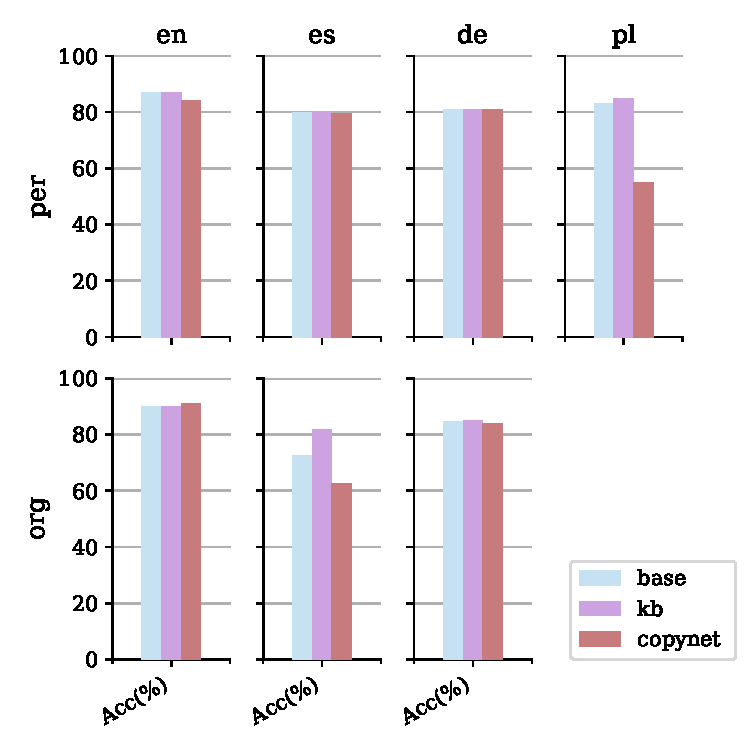
\includegraphics{yes-no_silver_results.pdf}}
    \caption{}
    \end{subfigure}
    \begin{subfigure}{0.59\linewidth}
    \resizebox{\textwidth}{!}{
    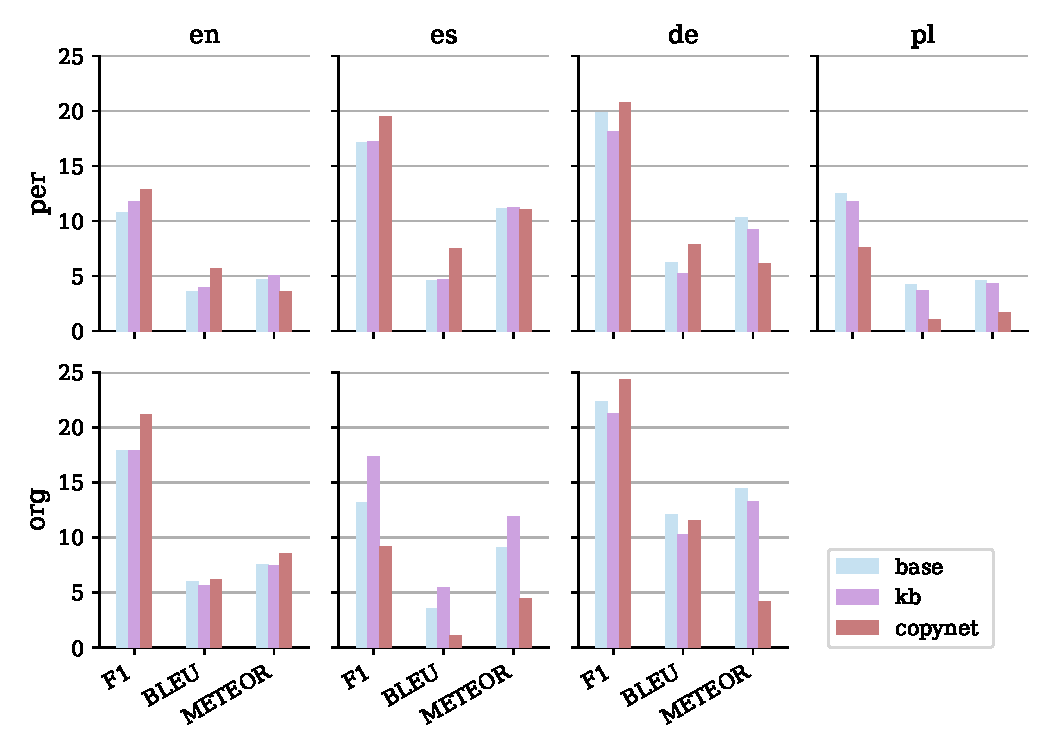
\includegraphics{generation_silver_results.pdf}}
    \caption{}
    \end{subfigure}
    \caption{(a) Evaluation of (a) the models' ability to correctly decide when an appositive is due, (b) generated predictions for positive test instances. Measured on the News test set. }
    \label{fig:silver}
\end{figure*}

The numbers behind the results from Figures~\ref{fig:gold} and~\ref{fig:silver} are shown in Tables~\ref{tab:gold_results} and ~\ref{tab:silver_results}, respectively.

\begin{table*}[]
    \centering
    \begin{tabular}{cllllllll}
        && Acc & F1 & BLEU & METEOR\\
        \hline
        \multirow{3}{*}{\rotatebox{90}{\textsc{en-per}}}&always yes &0.5&0.0&0.0&0.0\\
        &base &71.91&0.72&1.03&2.96\\
        &kb &71.73&0.73&1.03&2.9\\
        &copynet &70.19&0.71&2.45&2.24\\
        \hline
        \multirow{3}{*}{\rotatebox{90}{\textsc{en-org}}}&always yes &0.5&0.0&0.0&0.0\\
        &base &68.09&0.74&0.23&1.61\\
        &kb &66.58&0.74&0.21&1.58\\
        &copynet &65.98&0.73&0.52&1.37\\
        \hline
        \multirow{3}{*}{\rotatebox{90}{\textsc{es-per}}}&always yes &0.58&0.0&0.0&0.0\\
        &base &62.84&0.67&1.24&5.44\\
        &kb &61.18&0.68&0.79&4.79\\
        &copynet &64.08&0.67&2.2&4.36\\
        \hline
        \multirow{3}{*}{\rotatebox{90}{\textsc{es-org}}}&always yes &0.4&0.0&0.0&0.0\\
        &base &47.39&0.68&1.32&5.64\\
        &kb &60.91&0.71&2.02&6.83\\
        &copynet &33.57&0.62&0.33&2.77\\
        \hline
        \multirow{3}{*}{\rotatebox{90}{\textsc{de-per}}}&always yes &0.54&0.0&0.0&0.0\\
        &base &62.94&0.67&0.8&3.19\\
        &kb &63.47&0.68&0.75&2.84\\
        &copynet &67.63&0.69&1.75&1.76\\
        \hline
        \multirow{3}{*}{\rotatebox{90}{\textsc{de-org}}}&always yes &0.46&0.0&0.0&0.0\\
        &base &62.77&0.72&0.54&3.21\\
        &kb &65.13&0.73&0.19&3.47\\
        &copynet &62.22&0.72&0.43&1.08\\
        \hline
        \multirow{3}{*}{\rotatebox{90}{\textsc{pl-per}}}&always yes &0.54&0.0&0.0&0.0\\
        &base &72.83&0.78&0.16&0.09\\
        &kb &73.8&0.77&0.06&0.13\\
        &copynet &2.75&0.58&0.0&0.12\\
    \end{tabular}
    \caption{Evaluation of the models' ability to correctly decide when an appositive is due and of generated predictions for positive test instances. Measured on the News test set. }
    \label{tab:gold_results}
\end{table*}

\begin{table*}[]
    \centering
    \begin{tabular}{cllllllll}
    \hline
    \multirow{3}{*}{\rotatebox{90}{\textsc{en-per}}}&base &85.42&0.87&3.59&4.7\\
    &kb &85.32&0.87&3.94&5.07\\
    &copynet &81.95&0.84&5.7&3.57\\
    \hline
    \multirow{3}{*}{\rotatebox{90}{\textsc{en-org}}}&base &89.47&0.9&5.99&7.54\\
    &kb &89.43&0.9&5.65&7.49\\
    &copynet &89.17&0.91&6.17&8.53\\
    \hline
    \multirow{3}{*}{\rotatebox{90}{\textsc{es-per}}}&base &78.49&0.8&4.57&11.17\\
    &kb &78.73&0.8&4.71&11.19\\
    &copynet &79.1&0.8&7.54&11.04\\
    \hline
    \multirow{3}{*}{\rotatebox{90}{\textsc{es-org}}}&base &61.63&0.73&3.58&9.07\\
    &kb &80.69&0.82&5.45&11.92\\
    &copynet &46.91&0.62&1.14&4.46\\
    \hline
    \multirow{3}{*}{\rotatebox{90}{\textsc{de-per}}}&base &79.28&0.81&6.19&10.35\\
    &kb &80.09&0.81&5.24&9.19\\
    &copynet &80.12&0.81&7.85&6.11\\
    \hline
    \multirow{3}{*}{\rotatebox{90}{\textsc{de-org}}}&base &84.09&0.85&12.04&14.45\\
    &kb &84.58&0.85&10.28&13.31\\
    &copynet &82.07&0.84&11.57&4.19\\
    \hline
    \multirow{3}{*}{\rotatebox{90}{\textsc{pl-per}}}&base &82.67&0.83&4.23&4.61\\
    &kb &84.46&0.85&3.67&4.29\\
    &copynet &24.49&0.55&1.1&1.71\\
    \end{tabular}
    \caption{Evaluation of the models' ability to correctly decide when an appositive is due and of generated predictions for positive test instances. Measured on the Wiki test set. }
    \label{tab:silver_results}
\end{table*}

\subsection{Ranking paradigm study}
\label{taste_test}
Figure~\ref{fig:tastetest} shows an example prompt from the blind taste test. Instances where either the true appositive was empty or the predicted one was empty were included in the the study, but instances where both were empty were excluded, as the comparison would not have been meaningful in this case. The average time for completing a HIT was 53 seconds.
\begin{figure}
    \centering
    \resizebox{0.55\linewidth}{!}{
    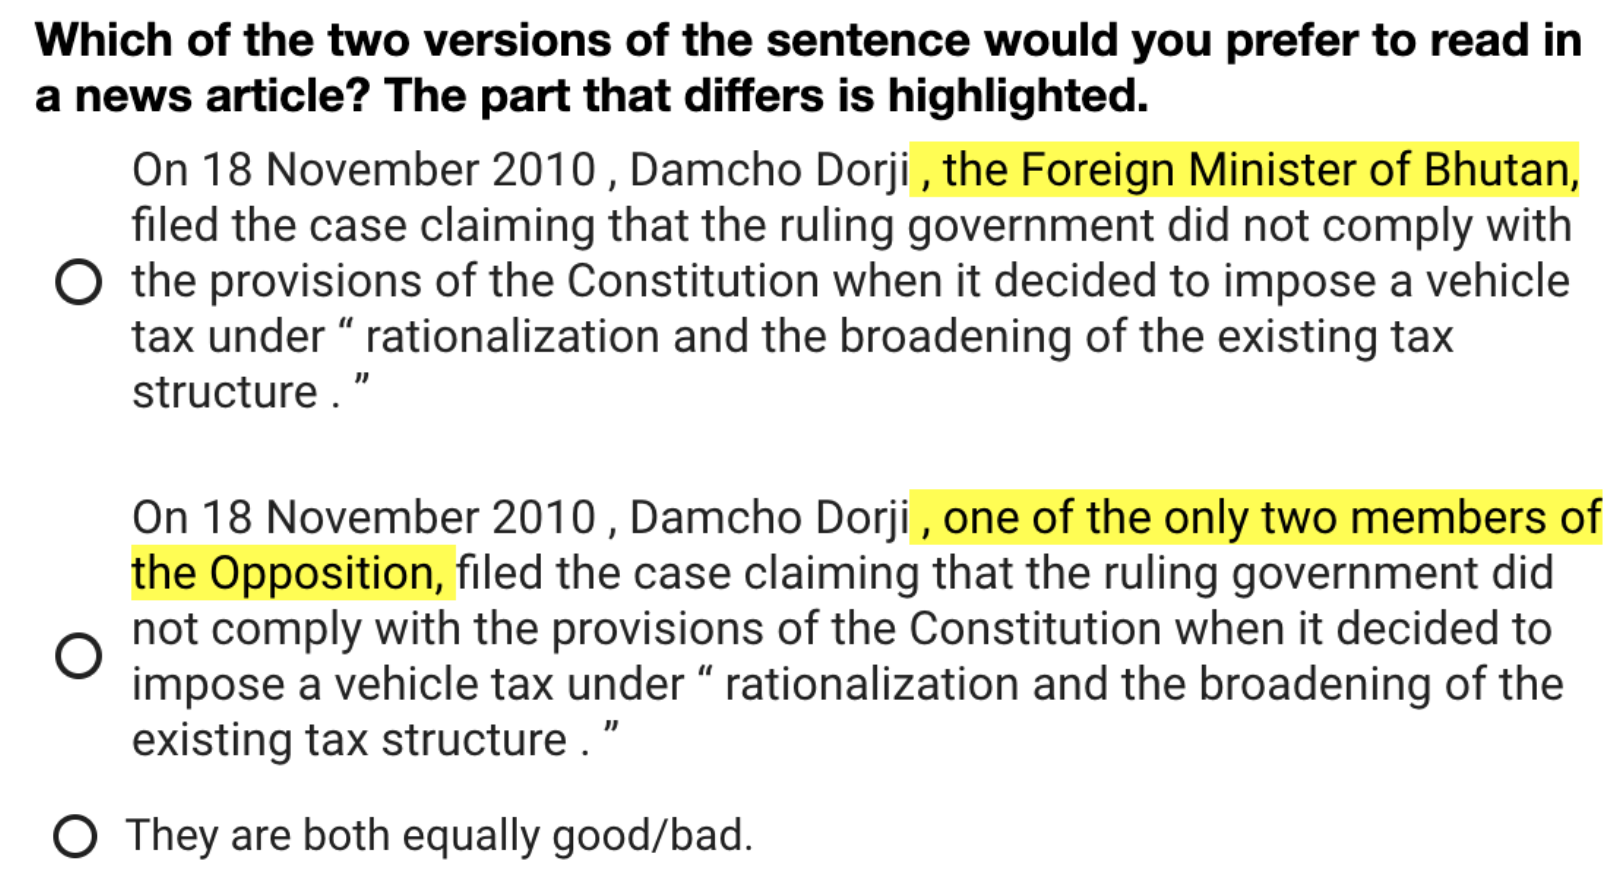
\includegraphics{tastetest.png}}
    \caption{Prompt for manual evaluation.}
    \label{fig:tastetest}
\end{figure}